\documentclass[10pt]{article}
\usepackage[utf8]{inputenc}
\usepackage[T1]{fontenc}
\usepackage{amsmath}
\usepackage{amsfonts}
\usepackage{amssymb}
\usepackage[version=4]{mhchem}
\usepackage{stmaryrd}
\usepackage{graphicx}
\usepackage[export]{adjustbox}
\graphicspath{ {./images/} }
\usepackage{caption}

\begin{document}
\captionsetup{singlelinecheck=false}
\section*{JEE-MAIN EXAMINATION - APRIL 2025}
(HELD ON MONDAY 07 \(^{\text {th }}\) APRIL 2025)\\
TIME : 9:00 AM TO 12:00 NOON

\section*{PHYSICS}
\section*{SECTION-A}
\begin{enumerate}
  \setcounter{enumi}{25}
  \item Two harmonic waves moving in the same direction superimpose to form a wave \(\mathrm{x}=\mathrm{a} \cos (1.5 \mathrm{t}) \cos (50.5 \mathrm{t})\) where \(t\) is in seconds. Find the period with which they beat (close to nearest integer)\\
(1) 6 s\\
(2) 4 s\\
(3) 1 s\\
(4) 2 s
\end{enumerate}

Ans. (4)\\
Sol. The given equation can be written as\\
\(x=\frac{a}{2} \cos [1.5+50.5] t+\frac{a}{2} \cos [50.5-1.5]\)\\
\(x=\frac{a}{2} \cos [52 t]+\frac{a}{2} \cos [49 t]\)\\
Here, \(2 \pi \mathrm{f}_{1} \& 2 \pi \mathrm{f}_{2}=49\)\\
\(\mathrm{f}_{1}=\frac{52}{2 \pi}, \mathrm{f}_{2}=\frac{49}{2 \pi}\)\\
\(\therefore \mathrm{f}_{\text {Beat }}=\mathrm{f}_{1}-\mathrm{f}_{2}=\frac{3}{2 \pi} \mathrm{~Hz}\)\\
\(\therefore \mathrm{T}_{\text {Beat }}=\frac{1}{\mathrm{f}_{\text {Beat }}}=\frac{2 \pi}{3} \sec\)\\
\(=2.09 \mathrm{sec} \approx 2 \mathrm{sec}\)\\
27. Two plane polarized light waves combine at a certain point whose electric field components are\\
\(\mathrm{E}_{1}=\mathrm{E}_{0} \sin \omega \mathrm{t}\)\\
\(\mathrm{E}_{2}=\mathrm{E}_{0} \sin \left(\omega \mathrm{t}+\frac{\pi}{3}\right)\)\\
Find the amplitude of the resultant wave.\\
(1) 0.9 E\\
(2) \(\mathrm{E}_{0}\)\\
(3) \(1.7 \mathrm{E}_{0}\)\\
(4) \(3.4 \mathrm{E}_{0}\)

Ans. (3)

\section*{TEST PAPER WITH SOLUTION}
Sol. \(\mathrm{E}=\sqrt{\left(\mathrm{E}_{0}\right)^{2}+\left(\mathrm{E}_{0}\right)^{2}+2\left(\mathrm{E}_{0}\right)\left(\mathrm{E}_{0}\right) \cos \frac{\pi}{3}}\)\\
\(\mathrm{E}=\sqrt{2 \mathrm{E}_{0}^{2}+\mathrm{E}_{0}^{2}}=\sqrt{3} \mathrm{E}_{0}=1.73 \mathrm{E}_{0}\)\\
28. A wire of resistance \(R\) is bent into a triangular pyramid as shown in figure with each segment having same length. The resistance between points \(A\) and \(B\) is \(R / n\). The value of \(n\) is :\\
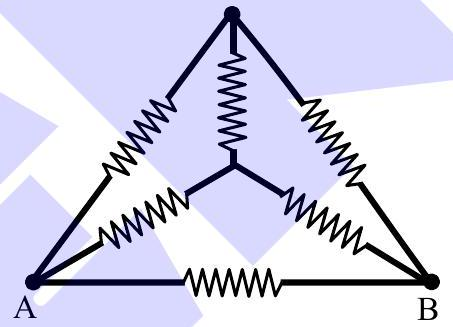
\includegraphics[max width=\textwidth, center]{2025_10_03_eb801c1f491f312ab0d3g-1}\\
(1) 16\\
(2) 14\\
(3) 10\\
(4) 12

Ans. (4)\\
Sol. As \(r=\frac{R}{6}\)\\
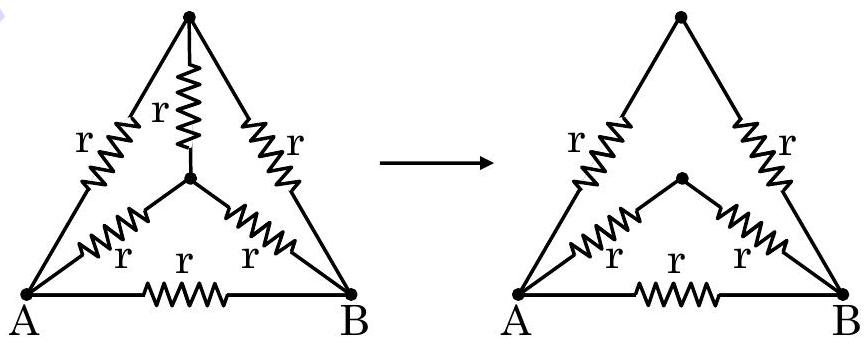
\includegraphics[max width=\textwidth, center]{2025_10_03_eb801c1f491f312ab0d3g-1(1)}\\
(As balanced wheat stone bridge is formed)\\
Now, Equivalent resistance between A and B can be written as

\[
\begin{aligned}
& \frac{1}{R_{A B}}=\frac{1}{2 r}+\frac{1}{2 r}+\frac{1}{r}=\frac{2}{r} \\
& R_{A B}=\frac{R}{12}
\end{aligned}
\]

\begin{enumerate}
  \setcounter{enumi}{28}
  \item Uniform magnetic fields of different strengths ( \(B_{1}\) and \(\mathrm{B}_{2}\) ), both normal to the plane of the paper exist as shown in the figure. A charged particle of mass m and charge q , at the interface at an instant, moves into the region 2 with velocity \(v\) and returns to the interface. It continues to move into region 1 and finally reaches the interface. What is the displacement of the particle during this movement along the interface ?
\end{enumerate}

\[
\begin{aligned}
& \times \times \times \times \times \times \times \times \times \\
& \times \times \times \times \mathrm{B}_{1 \times \times \times} \times \text { Region } 1 \\
& \frac{\mathrm{Interface}}{\times \times \times \times \times} \times \times \times \times \\
& \times \times \times \times \mathrm{B}_{2} \times \times \times
\end{aligned} \text { Region } 2
\]

(Consider the velocity of the particle to be normal to the magnetic field and \(\mathrm{B}_{2}>\mathrm{B}_{1}\) )\\
(1) \(\frac{\mathrm{m} v}{\mathrm{qB}_{1}}\left(1-\frac{\mathrm{B}_{2}}{\mathrm{~B}_{1}}\right) \times 2\)\\
(2) \(\frac{m v}{q B_{1}}\left(1-\frac{B_{1}}{B_{2}}\right)\)\\
(3) \(\frac{m v}{q B_{1}}\left(1-\frac{B_{2}}{B_{1}}\right)\)\\
(4) \(\frac{m v}{q B_{1}}\left(1-\frac{B_{1}}{B_{2}}\right) \times 2\)

Ans. (4)\\
Sol. As \(\overrightarrow{\mathrm{v}}\) is \(\perp\) to \(\overrightarrow{\mathrm{B}}\), so charge particle will move in circular path, whose radius is given by\\
\(\mathrm{R}=\frac{\mathrm{mv}}{\mathrm{qB}}\)\\
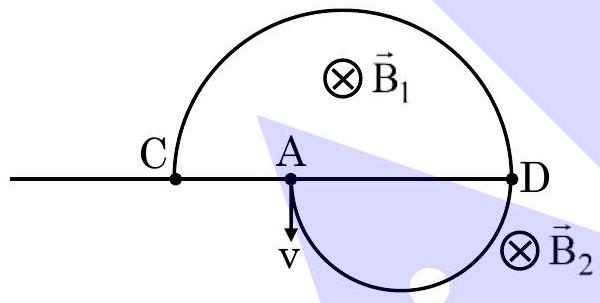
\includegraphics[max width=\textwidth, center]{2025_10_03_eb801c1f491f312ab0d3g-2(2)}

Starting point \(\rightarrow \mathrm{A}\)\\
Ending point \(\rightarrow \mathrm{C}\)\\
\(\therefore\) Net displacement \(=\mathrm{AC}\)\\
\(\mathrm{AC}=\mathrm{CD}-\mathrm{AD}\)\\
\(\mathrm{AC}=\frac{2 \mathrm{mv}}{\mathrm{qB}_{1}}-\frac{2 \mathrm{mv}}{\mathrm{qB}_{2}}\)\\
\(\mathrm{AC}=\frac{2 \mathrm{mv}}{\mathrm{qB}_{1}}\left[1-\frac{\mathrm{B}_{1}}{\mathrm{~B}_{2}}\right]\)\\
30. If \(\in_{0}\) denotes the permittivity of free space and \(\Phi_{E}\) is the flux of the electric field through the area bounded by the closed surface, then dimension of \(\left(\epsilon_{0} \frac{\mathrm{~d} \phi_{\mathrm{E}}}{\mathrm{dt}}\right)\) are that of :\\
(1) Electric field\\
(2) Electric potential\\
(3) Electric charge\\
(4) Electric current

Ans. (4)\\
Sol. We know that formula for displacement current is given by\\
\(\mathrm{id}=\varepsilon_{0} \frac{\mathrm{~d} \phi_{\varepsilon}}{\mathrm{dt}}\)\\
31. A rod of length 5 L is bent right angle keeping one side length as 2 L .\\
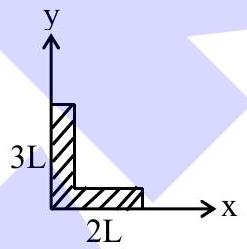
\includegraphics[max width=\textwidth, center]{2025_10_03_eb801c1f491f312ab0d3g-2}

The position of the centre of mass of the system:\\
(Consider L = 10 cm )\\
(1) \(2 \hat{i}+3 \hat{j}\)\\
(2) \(3 \hat{i}+7 \hat{j}\)\\
(3) \(5 \hat{i}+8 \hat{j}\)\\
(4) \(4 \hat{i}+9 \hat{j}\)

Ans. (4)\\
Sol.\\
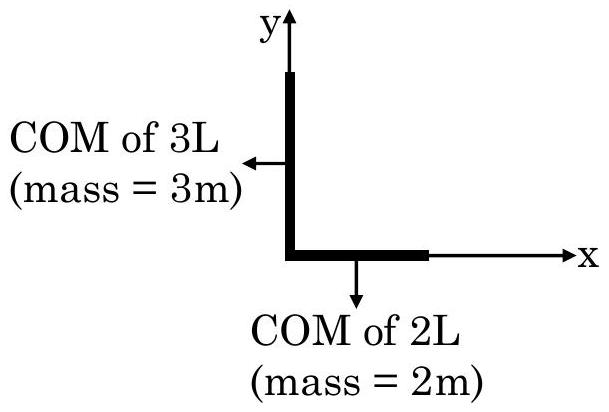
\includegraphics[max width=\textwidth, center]{2025_10_03_eb801c1f491f312ab0d3g-2(1)}\\
\(\mathrm{x}_{\text {com }}=\frac{2 \mathrm{~m}(10)+3 \mathrm{~m}(0)}{5 \mathrm{~m}}=4 \mathrm{~cm}\)\\
\(\mathrm{y}_{\text {com }}=\frac{2 \mathrm{~m}(0)+3 \mathrm{~m}(15)}{5 \mathrm{~m}}=9 \mathrm{~cm}\)\\
\(\overrightarrow{\mathrm{r}}_{\text {com }}=4 \hat{\mathrm{i}}+9 \hat{\mathrm{j}}\)\\
32. The percentage increase in magnetic field (B) when space within a current carrying solenoid is filled with magnesium (magnetic susceptibility \(\left.\chi_{\mathrm{mg}}=1.2 \times 10^{-5}\right)\) is :\\
(1) \(\frac{6}{5} \times 10^{-3} \%\)\\
(2) \(\frac{5}{6} \times 10^{-5} \%\)\\
(3) \(\frac{5}{6} \times 10^{-4} \%\)\\
(4) \(\frac{5}{3} \times 10^{-5} \%\)

Ans. (1)\\
Sol. \% change in \(\mathrm{B}=\frac{\mathrm{B}_{\text {new }}-\mathrm{B}_{\text {old }}}{\mathrm{B}_{\text {old }}} \times 100 \%\)\\
\(=\frac{\mu \mathrm{ni}-\mu_{0} \mathrm{ni}}{\mu_{0} \mathrm{ni}} \times 100 \%=\frac{\left(\mu-\mu_{0}\right)}{\mu_{0}} \times 100 \%\)\\
\(=\frac{\left(\mu_{0} \mu_{\mathrm{r}}-\mu_{0}\right)}{\mu_{0}} \times 100 \%\)\\
\(=\left(\mu_{\mathrm{r}}-1\right) \times 100 \%\)\\
\(=\chi_{\mathrm{n}} \times 100 \%\)\\
\(=1.2 \times 10^{-3} \%\)\\
33. A lens having refractive index 1.6 has focal length of 12 cm , when it is in air. Find the focal length of the lens when it is placed in water.\\
(Take refractive index of water as 1.28 )\\
(1) 355 mm\\
(2) 288 mm\\
(3) 555 mm\\
(4) 655 mm

Ans. (2)\\
Sol. As we know,\\
\(\frac{1}{\mathrm{f}}=\left[\frac{\mu_{\mathrm{L}}}{\mu_{\mathrm{m}}}-1\right]\left[\frac{1}{\mathrm{R}_{1}}-\frac{1}{\mathrm{R}_{2}}\right]\)\\
For air \(\mu_{\mathrm{m}}=1\)\\
\(\frac{1}{12}=[1.6-1]\left[\frac{1}{\mathrm{R}_{1}}-\frac{1}{\mathrm{R}_{2}}\right]\)\\
\(\frac{1}{12}=\frac{6}{10}\left[\frac{1}{\mathrm{R}_{1}}-\frac{1}{\mathrm{R}_{2}}\right]\)\\
\(\left[\frac{1}{\mathrm{R}_{1}}-\frac{1}{\mathrm{R}_{2}}\right]=\frac{10}{72}\)\\
For water\\
\(\frac{1}{\mathrm{f}}=\left[\frac{1.6}{1.28}-1\right]\left[\frac{10}{72}\right]=\frac{32}{128} \times \frac{10}{72}\)\\
\(\frac{1}{\mathrm{f}}=\frac{1}{4} \times \frac{10}{72}\)\\
\(\mathrm{f}=28.8 \mathrm{~cm}\)\\
\(\mathrm{f}=288 \mathrm{~mm}\)\\
34. An ac current is represented as\\
\(\mathrm{i}=5 \sqrt{2}+10 \cos \left(650 \pi \mathrm{t}+\frac{\pi}{6}\right)\) Amp\\
The r.m.s value of the current is\\
(1) 50 Amp\\
(2) 100 Amp\\
(3) 10 Amp\\
(4) \(5 \sqrt{2} \mathrm{Amp}\)

Ans. (3)\\
Sol. \(\quad i=5 \sqrt{2}+10 \cos \left(650 \pi t+\frac{\pi}{6}\right)\)\\
\(i^{2}=50+100 \cos ^{2}\left(650 \pi t+\frac{\pi}{6}\right)\)\\
\(+(2)(5 \sqrt{2})(10) \cos \left(650 \pi t+\frac{\pi}{6}\right)\)\\
\(\left\langle\mathrm{i}^{2}\right\rangle=50+\frac{100}{2}+0\)\\
\(\left\langle\mathrm{i}^{2}\right\rangle=100\)\\
\(<\mathrm{i}>=10 \mathrm{Amp}\).\\
35. Two thin convex lenses of focal lengths 30 cm and 10 cm are placed coaxially, 10 cm apart. The power of this combination is :\\
(1) 5 D\\
(2) 1 D\\
(3) 20 D\\
(4) 10 D

Ans. (4)\\
Sol. \(\mathrm{f}_{1}=30 \mathrm{~cm}, \mathrm{f}_{2}=10 \mathrm{~cm}\)\\
\(\frac{1}{\mathrm{f}_{\mathrm{eq}}}=\frac{1}{\mathrm{f}_{1}}+\frac{1}{\mathrm{f}_{2}}-\frac{\mathrm{d}}{\mathrm{f}_{1} \mathrm{f}_{2}}, \mathrm{~d}=\) distance between lens\\
\(\frac{1}{\mathrm{f}_{\text {eq }}}=\frac{1}{0.3}+\frac{1}{0.1}-\frac{0.1}{(0.3)(0.1)}\)\\
\(\frac{1}{\mathrm{f}_{\text {eq }}}=\frac{1}{0.1}\)\\
Power \(=\frac{1}{\mathrm{f}_{\mathrm{eq}}}=10 \mathrm{D}\)\\
36. In the following circuit, the reading of the ammeter will be (Take Zener breakdown voltage \(=4 \mathrm{~V}\) )\\
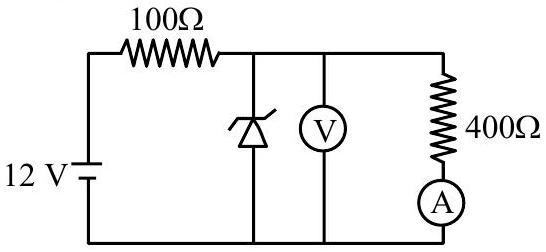
\includegraphics[max width=\textwidth, center]{2025_10_03_eb801c1f491f312ab0d3g-4(1)}\\
(1) 24 mA\\
(2) 80 mA\\
(3) 10 mA\\
(4) 60 mA

Ans. (3)\\
Sol.\\
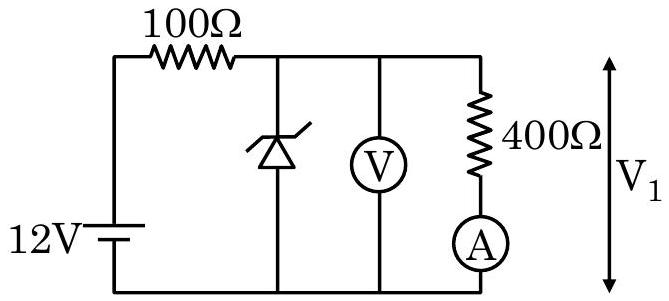
\includegraphics[max width=\textwidth, center]{2025_10_03_eb801c1f491f312ab0d3g-4}

\[
V_{1}=\frac{400}{100+400} \times 12 V=\frac{4}{5} \times 12=\frac{48}{5} V
\]

here, \(\mathrm{V}_{1}>\mathrm{V}_{\mathrm{z}},\left(\mathrm{V}_{\mathrm{z}}=\right.\) Zener Voltage \()\)\\
So, Zener breakdown will be take place\\
So, voltage across \(400 \Omega\) will be 4 V\\
\(\mathrm{I}=\frac{4}{400} \mathrm{~A}=\frac{1}{100 \mathrm{~A}}=10 \mathrm{~mA}\)\\
37. Two projectiles are fired from ground with same initial speeds from same point at angles ( \(45^{\circ}+\alpha\) ) and ( \(45^{\circ}-\alpha\) ) with horizontal direction. The ratio of their times of flights is\\
(1) 1\\
(2) \(\frac{1-\tan \alpha}{1+\tan \alpha}\)\\
(3) \(\frac{1+\sin 2 \alpha}{1-\sin 2 \alpha}\)\\
(4) \(\frac{1+\tan \alpha}{1-\tan \alpha}\)

Ans. (4)\\
Sol. \(\theta_{1}=45+\alpha ; \theta_{2}=45-\alpha\)\\
Time of flight, \(\mathrm{T}=\frac{2 \mathrm{v} \sin \theta}{\mathrm{g}}\)\\
\(\frac{T_{1}}{T_{2}}=\frac{\sin (45+\alpha)}{\sin (45-\alpha)}\)\\
\(\frac{\mathrm{T}_{1}}{\mathrm{~T}_{2}}=\frac{\frac{1}{\sqrt{2}} \cos \alpha+\frac{1}{\sqrt{2}} \sin \alpha}{\frac{1}{\sqrt{2}} \cos \alpha-\frac{1}{\sqrt{2}} \sin \alpha}\)\\
\(\frac{\mathrm{T}_{1}}{\mathrm{~T}_{2}}=\frac{\cos \alpha+\sin \alpha}{\cos \alpha-\sin \alpha}=\frac{1+\tan \alpha}{1-\tan \alpha}\)\\
38. Match the List-I with List-II

\begin{center}
\begin{tabular}{|l|l|l|l|}
\hline
\multicolumn{2}{|c|}{List-I} & \multicolumn{2}{|c|}{List-II} \\
\hline
A. & Triatomic rigid gas & I. & \(\frac{\mathrm{C}_{\mathrm{P}}}{\mathrm{C}_{\mathrm{V}}}=\frac{5}{3}\) \\
\hline
B. & Diatomic non-rigid gas & II. & \(\frac{\mathrm{C}_{\mathrm{P}}}{\mathrm{C}_{\mathrm{V}}}=\frac{7}{5}\) \\
\hline
C. & Monoatomic gas & III. & \(\frac{\mathrm{C}_{\mathrm{P}}}{\mathrm{C}_{\mathrm{V}}}=\frac{4}{3}\) \\
\hline
D. & Diatomic rigid gas & IV & \(\frac{\mathrm{C}_{\mathrm{P}}}{\mathrm{C}_{\mathrm{V}}}=\frac{9}{7}\) \\
\hline
\end{tabular}
\end{center}

Choose the correct answer from the options given below :\\
(1) A-III, B-IV, C-I, D-II\\
(2) A-III, B-II, C-IV, D-I\\
(3) A-II, B-IV, C-I, D-III\\
(4) A-IV, B-II, C-III, D-I

Ans. (1)\\
Sol. \(\quad \gamma=1+\frac{2}{\mathrm{f}}\)\\
\(\mathrm{f}=6\), Triatomic rigid gas\\
\(\mathrm{f}=7\), Diatomic non-rigid gas\\
\(\mathrm{f}=5\), Diatomic rigid gas\\
\(\mathrm{f}=3\), monoatomic rigid gas\\
\(\gamma=1+\frac{2}{6}=\frac{4}{3}\) (Triatomic)\\
\(\gamma=1+\frac{2}{7}=\frac{9}{7}\) (Diatomic, non-rigid)\\
\(\gamma=1+\frac{2}{5}=\frac{7}{5}\) (Diatomic, rigid)\\
\(\gamma=1+\frac{2}{3}=\frac{5}{3}\) (Monoatomic, rigid)\\
A-III, B-IV, C-I, D-II\\
39. A cubic block of mass \(m\) is sliding down on an inclined plane at \(60^{\circ}\) with an acceleration of \(\frac{\mathrm{g}}{2}\), the value of coefficient of kinetic friction is\\
(1) \(\sqrt{3}-1\)\\
(2) \(\frac{\sqrt{3}}{2}\)\\
(3) \(\frac{\sqrt{2}}{3}\)\\
(4) \(1-\frac{\sqrt{3}}{2}\)

Ans. (1)\\
Sol.\\
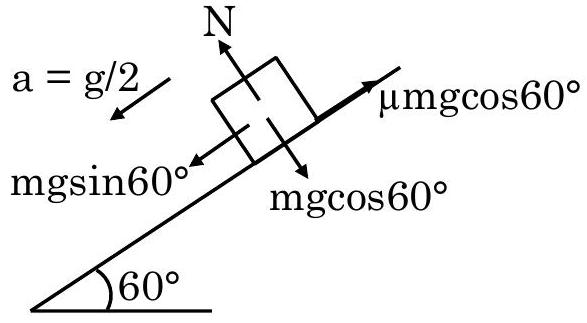
\includegraphics[max width=\textwidth, center]{2025_10_03_eb801c1f491f312ab0d3g-5(4)}\\
\(\operatorname{mgsin} 60^{\circ}-\mu \operatorname{mgcos} 60^{\circ}=\) ma\\
\(g \sin 60-\mu g \cos 60=\frac{g}{2}\)\\
\(\frac{\sqrt{3}}{2}-\frac{\mu}{2}=\frac{1}{2}\)\\
\(\mu=\sqrt{3}-1\)\\
40. In a hydrogen like ion, the energy difference between the \(2^{\text {nd }}\) excitation energy state and ground is 108.8 eV . The atomic number of the ion is\\
(1) 4\\
(2) 2\\
(3) 1\\
(4) 3

Allen Ans. (4)\\
NTA Ans. (2)\\
Sol. \(\quad \Delta \mathrm{E}=13.6 \mathrm{z}^{2}\left[\frac{1}{\mathrm{n}_{1}^{2}}-\frac{1}{\mathrm{n}_{2}^{2}}\right]\)\\
\((13.6) \mathrm{z}^{2}\left[\frac{1}{1}-\frac{1}{9}\right]=108.8\)\\
\(\frac{(13.6)(8)}{9}\left(z^{2}\right)=108.8\)\\
\(\mathrm{z}=3\)\\
41. For a hydrogen atom, the ratio of the largest wavelength of Lyman series to that of the Balmer series is.\\
(1) \(5: 36\)\\
(2) \(5: 27\)\\
(3) \(3: 4\)\\
(4) \(27: 5\)

Ans. (2)\\
Sol. Lyman\\
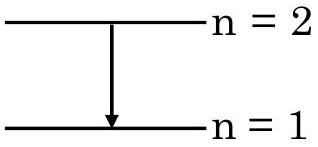
\includegraphics[max width=\textwidth, center]{2025_10_03_eb801c1f491f312ab0d3g-5(3)}\\
\(\frac{1}{\lambda_{1}}=\mathrm{R}\left[\frac{1}{1}-\frac{1}{4}\right]=\frac{3 \mathrm{R}}{4}\)\\
\(\lambda_{1}=\frac{4}{3 \mathrm{R}}\)\\
and Balmer\\
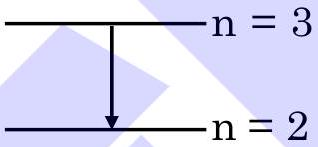
\includegraphics[max width=\textwidth, center]{2025_10_03_eb801c1f491f312ab0d3g-5(2)}\\
\(\frac{1}{\lambda_{2}}=\mathrm{R}\left[\frac{1}{4}-\frac{1}{9}\right]=\frac{5 \mathrm{R}}{36}\)\\
\(\lambda_{2}=\frac{36}{5 R}\)\\
Then, \(\frac{\lambda_{1}}{\lambda_{2}}=\frac{5}{27}\)\\
42. A particle of charge q , mass m and kinetic energy E enters in magnetic field perpendicular to its velocity and undergoes a circular arc of radius(r). Which of the following curves represents the variation of \(r\) with \(E\) ?

\begin{figure}[h]
\begin{center}
\captionsetup{labelformat=empty}
\caption{(1)}
  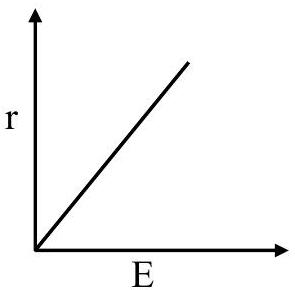
\includegraphics[width=\textwidth]{2025_10_03_eb801c1f491f312ab0d3g-5(6)}
\end{center}
\end{figure}

\begin{figure}[h]
\begin{center}
\captionsetup{labelformat=empty}
\caption{(2)}
  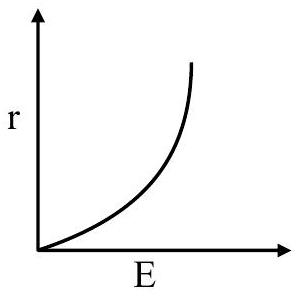
\includegraphics[width=\textwidth]{2025_10_03_eb801c1f491f312ab0d3g-5(5)}
\end{center}
\end{figure}

\begin{figure}[h]
\begin{center}
\captionsetup{labelformat=empty}
\caption{(3)}
  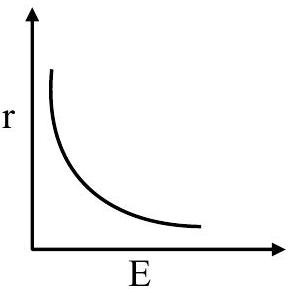
\includegraphics[width=\textwidth]{2025_10_03_eb801c1f491f312ab0d3g-5}
\end{center}
\end{figure}

\begin{figure}[h]
\begin{center}
\captionsetup{labelformat=empty}
\caption{(4)}
  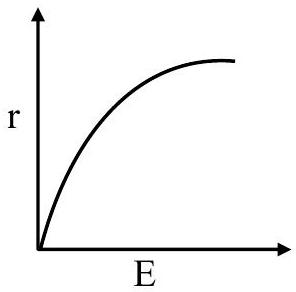
\includegraphics[width=\textwidth]{2025_10_03_eb801c1f491f312ab0d3g-5(1)}
\end{center}
\end{figure}

Ans. (4)

Sol.\\
\(\mathrm{v} \uparrow \uparrow^{\mathrm{B}}\)\\
\(\frac{m v^{2}}{r}=q v B\)\\
\(\mathrm{mv}=\mathrm{qBr}\)\\
\(\mathrm{E}=\frac{1}{2} \mathrm{mv}^{2}\)\\
\(\mathrm{E}=\frac{1}{2} \mathrm{~m}\left(\frac{\mathrm{q}^{2} \mathrm{~B}^{2} \mathrm{r}^{2}}{\mathrm{~m}^{2}}\right)=\frac{\mathrm{q}^{2} \mathrm{~B}^{2} \mathrm{r}^{2}}{2 \mathrm{~m}}\)\\
\(\mathrm{E}=\left(\frac{\mathrm{q}^{2} \mathrm{~B}^{2}}{2 \mathrm{~m}}\right) \mathrm{r}^{2}\)\\
\(\mathrm{r}^{2} \propto \mathrm{E}\)\\
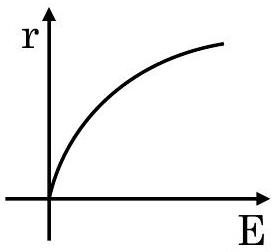
\includegraphics[max width=\textwidth, center]{2025_10_03_eb801c1f491f312ab0d3g-6}\\
43. An object of mass 1000 g experiences a time dependent force \(\overrightarrow{\mathrm{F}}=\left(2 \mathrm{t} \hat{\mathrm{i}}+3 \mathrm{t}^{2} \hat{\mathrm{j}}\right) \mathrm{N}\). The power generated by the force at time t is :\\
(1) \(\left(2 t^{2}+3 t^{3}\right) W\)\\
(2) \(\left(2 t^{2}+18 t^{3}\right) W\)\\
(3) \(\left(3 t^{3}+5 t^{5}\right) W\)\\
(4) \(\left(2 t^{3}+3 t^{5}\right) W\)

Ans. (4)\\
Sol. \(\overrightarrow{\mathrm{F}}=(2 t \hat{\mathrm{i}}+3 t \hat{\mathrm{j}}) \mathrm{N}\)\\
\(\mathrm{m}=1000 \mathrm{gm}=1 \mathrm{~kg}\)\\
\(\overrightarrow{\mathrm{F}}=\mathrm{ma}, \overrightarrow{\mathrm{a}}=2 \mathrm{t} \hat{\mathrm{i}}+3 \mathrm{t}^{2} \hat{\mathrm{j}}\)\\
\(\frac{\mathrm{d} \overrightarrow{\mathrm{v}}}{\mathrm{dt}}=2 \mathrm{t} \hat{\mathrm{i}}+3 \mathrm{t}^{2} \hat{\mathrm{j}}\)\\
\(\overrightarrow{\mathrm{v}}=\mathrm{t}^{2} \hat{\mathrm{i}}+\mathrm{t}^{3} \hat{\mathrm{j}}\)\\
Power, \(\mathrm{P}=\overrightarrow{\mathrm{F}} \cdot \overrightarrow{\mathrm{v}}\)\\
\(\mathrm{P}=\left(2 \mathrm{t} \hat{\mathrm{i}}+3 \mathrm{t}^{2} \hat{\mathrm{j}}\right) \cdot\left(\mathrm{t}^{2} \hat{\mathrm{i}}+\mathrm{t}^{3} \hat{\mathrm{j}}\right)\)\\
\(\mathrm{P}=\left(2 \mathrm{t}^{3}+3 \mathrm{t}^{5}\right) \mathrm{W}\)\\
44. Two wires A and B are made of same material having ratio of lengths \(\frac{L_{A}}{L_{B}}=\frac{1}{3}\) and their diameters ratio \(\frac{\mathrm{d}_{\mathrm{A}}}{\mathrm{d}_{\mathrm{B}}}=2\). If both the wires are stretched using same force, what would be the ratio of their respective elongations?\\
(1) \(1: 6\)\\
(2) \(1: 12\)\\
(3) \(3: 4\)\\
(4) \(1: 3\)

Ans. (2)\\
Sol. \(\frac{\mathrm{L}_{\mathrm{A}}}{\mathrm{L}_{\mathrm{B}}}=\frac{1}{3}\) and \(\frac{\mathrm{d}_{\mathrm{A}}}{\mathrm{d}_{\mathrm{B}}}=2\)\\
\(\Delta L_{A}=\frac{F_{A} L_{A}}{A_{A} Y_{A}}\) and \(\Delta L_{B}=\frac{F_{B} L_{B}}{A_{B} Y_{B}}\)\\
Given, \(\mathrm{F}_{\mathrm{A}}=\mathrm{F}_{\mathrm{B}}\) and \(\mathrm{Y}_{\mathrm{A}}=\mathrm{Y}_{\mathrm{B}}\)\\
\(\frac{\Delta L_{A}}{\Delta L_{B}}=\frac{\frac{F_{A} L_{A}}{A_{A} Y_{A}}}{\frac{F_{B} L_{B}}{A_{B} Y_{B}}}=\left(\frac{L_{A}}{L_{B}}\right)\left(\frac{A_{B}}{A_{A}}\right)\)\\
\(\frac{\Delta L_{A}}{\Delta L_{B}}=\left(\frac{L_{A}}{L_{B}}\right)\left(\frac{\frac{\pi}{4} d_{B}^{2}}{\frac{\pi}{4} d_{A}^{2}}\right)=\left(\frac{L_{A}}{L_{B}}\right)\left(\frac{d_{B}}{d_{A}}\right)^{2}\)\\
\(\frac{\Delta \mathrm{L}_{\mathrm{A}}}{\Delta \mathrm{L}_{\mathrm{B}}}=\left(\frac{1}{3}\right)\left(\frac{1}{2}\right)^{2}=\frac{1}{12}\)\\
45. Two charges \(\mathrm{q}_{1}\) and \(\mathrm{q}_{2}\) are separated by a distance of 30 cm . A third charge \(\mathrm{q}_{3}\) initially at ' C ' as shown in the figure, is moved along the circular path of radius 40 cm from C to D . If the difference in potential energy due to movement of \(\mathrm{q}_{3}\) from C to \(D\) is given by \(\frac{q_{3} K}{4 \pi \epsilon_{0}}\), the value of \(K\) is :\\
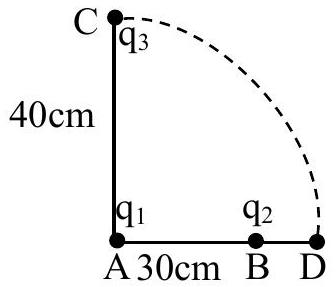
\includegraphics[max width=\textwidth, center]{2025_10_03_eb801c1f491f312ab0d3g-6(1)}\\
(1) \(8 q_{2}\)\\
(2) \(6 q_{2}\)\\
(3) \(8 q_{1}\)\\
(4) \(6 q_{1}\)

Ans. (1)

Sol. Potential at C\\
\(\mathrm{V}_{\mathrm{C}}=\frac{\mathrm{kq}_{1}}{0.4}+\frac{\mathrm{kq}_{2}}{0.5}\)\\
Potential at D\\
\(\mathrm{V}_{\mathrm{D}}=\frac{\mathrm{kq}_{1}}{0.4}+\frac{\mathrm{kq}_{2}}{0.1}\)\\
\(\Delta \mathrm{U}=\left(\mathrm{V}_{\mathrm{D}}-\mathrm{V}_{\mathrm{C}}\right)\left(\mathrm{q}_{3}\right)=\left(\frac{\mathrm{kq}_{2}}{0.1}-\frac{\mathrm{kq}_{2}}{0.5}\right)\left(\mathrm{q}_{3}\right)\)\\
\(\Delta U=8 k q_{2} q_{3}=\frac{8 q_{2} q_{3}}{4 \pi \varepsilon_{0}}\)

\section*{SECTION-B}
\begin{enumerate}
  \setcounter{enumi}{45}
  \item A,B and C are disc, solid sphere and spherical shell respectively with same radii and masses. These masses are placed as shown in figure.\\
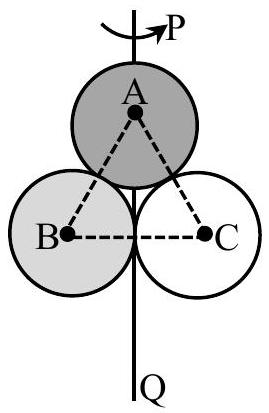
\includegraphics[max width=\textwidth, center]{2025_10_03_eb801c1f491f312ab0d3g-7(6)}
\end{enumerate}

The moment of inertia of the given system about PQ is \(\frac{\mathrm{X}}{15} \mathrm{I}\), where I is the moment of inertia of the disc about its diameter. The value of \(x\) is \(\_\_\_\_\) .\\
Ans. (199)

Sol.\\
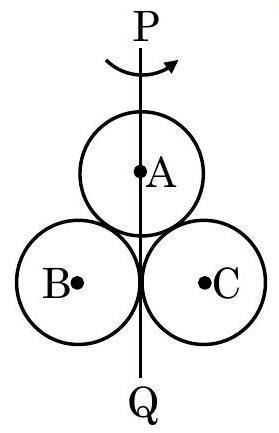
\includegraphics[max width=\textwidth, center]{2025_10_03_eb801c1f491f312ab0d3g-7(1)}

All bodies have same mass and same radius.\\
A \(\rightarrow\) Disc\\
\(\mathrm{B} \rightarrow\) Solid sphere\\
C \(\rightarrow\) Spherical shell\\
and, \(\mathrm{I}=\frac{\mathrm{MR}^{2}}{4}\)\\
\(\mathrm{I}_{\mathrm{PQ}}=\frac{\mathrm{MR}^{2}}{4}+\left(\frac{2}{5} \mathrm{MR}^{2}+\mathrm{MR}^{2}\right)+\left(\frac{2}{3} \mathrm{MR}^{2}+\mathrm{MR}^{2}\right)\)\\
\(\mathrm{I}_{\mathrm{PQ}}=\frac{15 \mathrm{MR}^{2}+24 \mathrm{MR}^{2}+60 \mathrm{MR}^{2}+40 \mathrm{MR}^{2}+60 \mathrm{MR}^{2}}{60}\)\\
\(\mathrm{I}_{\mathrm{PQ}}=\frac{199}{60} \mathrm{MR}^{2}=\frac{199}{15}\left(\frac{\mathrm{MR}^{2}}{4}\right)\)\\
\(=\frac{199}{15} \mathrm{I}\)\\
47. For ac circuit shown in figure, \(\mathrm{R}=100 \mathrm{k} \Omega\) and \(\mathrm{C}=100 \mathrm{pF}\) and the phase difference between \(\mathrm{V}_{\text {in }}\) and \(\left(V_{B}-V_{A}\right)\) is \(90^{\circ}\). The input signal frequency is \(10^{\mathrm{x}} \mathrm{rad} / \mathrm{sec}\), where ' x ' is \(\_\_\_\_\)\\
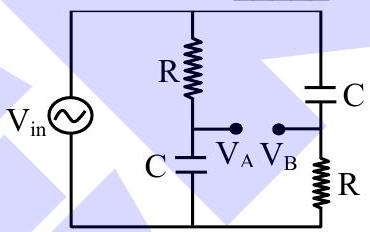
\includegraphics[max width=\textwidth, center]{2025_10_03_eb801c1f491f312ab0d3g-7}

Ans. (5)\\
Sol. Input voltage\\
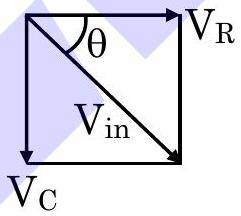
\includegraphics[max width=\textwidth, center]{2025_10_03_eb801c1f491f312ab0d3g-7(2)}\\
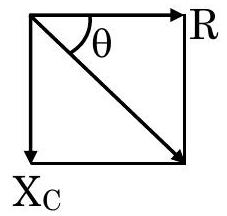
\includegraphics[max width=\textwidth, center]{2025_10_03_eb801c1f491f312ab0d3g-7(3)}\\
\(\mathbf{V}_{\mathbf{A}}-\mathbf{V}_{\mathbf{B}}:\)\\
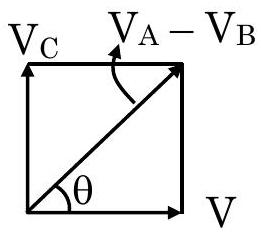
\includegraphics[max width=\textwidth, center]{2025_10_03_eb801c1f491f312ab0d3g-7(4)}\\
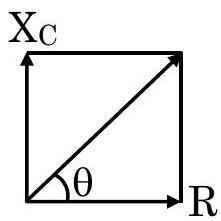
\includegraphics[max width=\textwidth, center]{2025_10_03_eb801c1f491f312ab0d3g-7(5)}\\
\(\theta+\theta=90^{\circ} ; \theta=45^{\circ}\)\\
\(\tan \theta=\frac{\mathrm{X}_{\mathrm{C}}}{\mathrm{R}}\)\\
\(\mathrm{X}_{\mathrm{C}}=\mathrm{R} \Rightarrow \frac{1}{\mathrm{~W}_{\mathrm{C}}}=\mathrm{R}\)\\
\(\mathrm{W}=\frac{1}{\mathrm{R}_{\mathrm{C}}}=\frac{1}{100 \times 10^{3} \times 100 \times 10^{-12}}\)\\
\(=\frac{10^{12}}{10^{7}}=10^{5}\)\\
48. A container contains a liquid with refractive index of 1.2 up to a height of 60 cm and another liquid having refractive index 1.6 is added to height H above first liquid. If viewed from above, the apparent shift in the position of bottom of container is 40 cm . The value of H is \(\_\_\_\_\) cm.\\
(Consider liquids are immisible)\\
Ans. (80)\\
Sol.\\
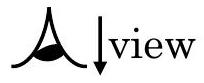
\includegraphics[max width=\textwidth, center]{2025_10_03_eb801c1f491f312ab0d3g-8(2)}\\
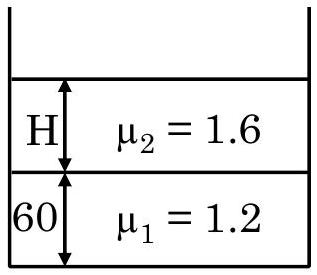
\includegraphics[max width=\textwidth, center]{2025_10_03_eb801c1f491f312ab0d3g-8}\\
\(\mathrm{y}=\) apparent depth of bottom\\
\(\frac{\mathrm{y}}{1}=\frac{\mathrm{H}}{1.6}+\frac{60}{1.2}\)\\
Shift = 40\\
\(H+60-y=40\)\\
\(\mathrm{H}+60-\frac{\mathrm{H}}{1.6}-\frac{60}{1.2}=40\)\\
\(\frac{6}{16} \mathrm{H}=30\)\\
\(\mathrm{H}=80 \mathrm{~cm}\)\\
49. A wire of length 10 cm and diameter 0.5 mm is used in a bulb. The temperature of the wire is \(1727^{\circ} \mathrm{C}\) and power radiated by the wire is 94.2 W . Its emissivity is \(\frac{\mathrm{X}}{8}\) where \(\mathrm{x}=\) \(\_\_\_\_\)\\
(Given \(\sigma=6.0 \times 10^{-8} \mathrm{~W} \mathrm{~m}^{-2} \mathrm{~K}^{-4}, \pi=3.14\) and assume that the emissivity of wire material is same at all wavelength. )

Ans. (5)

Sol. \(\mathrm{L}=10 \mathrm{~cm}, \mathrm{~d}=0.5 \mathrm{~mm}, \mathrm{~T}=1727^{\circ} \mathrm{C}=2000 \mathrm{~K}\)\\
Power, \(\mathrm{P}=94.2 \mathrm{~W}\)\\
\(\mathrm{P}=\varepsilon \sigma \mathrm{AT}^{4}\)\\
\(94.2=\varepsilon \times\left(6 \times 10^{-8}\right)(\pi \mathrm{dL})(2000)^{4}\)\\
\(94.2=\varepsilon \times\left(6 \times 10^{-8}\right)(3.14)(0.5)\left(10^{-3}\right)\)\\
\(\left(10 \times 10^{-2}\right)(2000)^{4}\)\\
\(\varepsilon=\frac{94.2}{(94.2)(16)}=\frac{5}{8}\)\\
50. An ideal gas has undergone through the cyclic process as shown in the figure. Work done by the gas in the entire cycle is \(\_\_\_\_\) \(\times 10^{-1} \mathrm{~J}\).\\
(Take \(\pi=3.14\) )\\
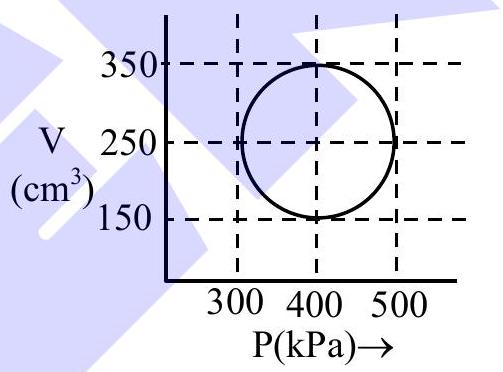
\includegraphics[max width=\textwidth, center]{2025_10_03_eb801c1f491f312ab0d3g-8(3)}

Ans. (314)\\
Sol.\\
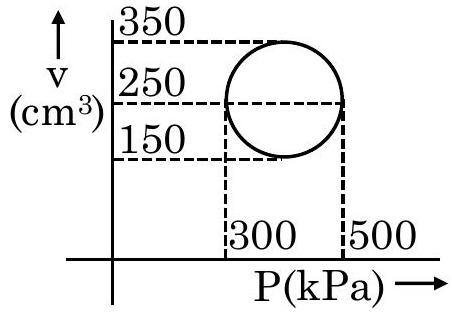
\includegraphics[max width=\textwidth, center]{2025_10_03_eb801c1f491f312ab0d3g-8(1)}

Area of circle, \(W=\frac{\pi}{4} d_{1} d_{2}\)\\
\(\mathrm{W}=\frac{\pi}{4}(500-300) \times 10^{3}(350-150) \times 10^{-6}\)\\
W = 31.4 Joule\\
\(\mathrm{W}=314 \times 10^{-1}\) Joule

\section*{Level up your prep for JEE with our LIVE JEE Courses!}
LIVE classes with top Kota faculty\\
ALLEN's study material\\
Tests with national benchmarking\\
ALLEN App Advantage: 24/7 doubt support, Custom Practice \& more

Enrol Now

\section*{ALLEN ONLINE}
\section*{Secure up to}
\section*{90\% scholarship on our Online Courses!}
\section*{based on your JEE Main 2025 scores!}
Enrol Now


\end{document}